\documentclass[12pt]{article}
%%%%%%%%%%%%%%%%%%%%%%%%%%%%%%%%%%%%%%%%%%%%%%%%%%%%%%%%%%%%%%%%%%%%%%%%%%%%%%%%%%%%%%%%%%%%%%%%%%%%%%%%%%%%%%%%%%%%%%%%%%%%%%%%%%%%%%%%%%%%%%%%%%%%%%%%%%%%%%%%%%%%%%%%%%%%%%%%%%%%%%%%%%%%%%%%%%%%%%%%%%%%%%%%%%%%%%%%%%%%%%%%%%%%%%%%%%%%%%%%%%%%%%%%%%%%
\usepackage{amsfonts}
\usepackage{eurosym}
\usepackage{geometry}
\usepackage{amsmath,amsthm,amssymb}
\usepackage{ulem} 
\usepackage{graphicx}
\usepackage{comment}
%\usepackage[sort,comma]{natbib}
\usepackage[utf8]{inputenc}
\usepackage{setspace}
\usepackage[backend=biber, style = apa]{biblatex}
\usepackage{placeins} % to separate sections

\usepackage{adjustbox}
\usepackage{array}
\usepackage{multirow}
\usepackage{graphicx}
\usepackage{subcaption}
\usepackage{pifont}
\usepackage{amssymb}
\usepackage{comment}
\usepackage[hang, flushmargin, bottom]{footmisc}
\usepackage{footnotebackref}
\usepackage{xcolor}
\usepackage{hyperref}
\usepackage{booktabs}
\usepackage{pifont}
\usepackage{caption}
\usepackage{float}
\usepackage{todonotes}
\setcounter{MaxMatrixCols}{10}


%\setlength{\bibsep}{0.3pt}
\setlength{\textfloatsep}{5pt}
\hypersetup{breaklinks=true,hypertexnames=false,colorlinks=true,citecolor = teal}
\captionsetup{font=normalsize}
\newcommand{\cmark}{\ding{51}}
\def\sym#1{\ifmmode^{#1}\else\(^{#1}\)\fi}
\renewcommand{\thetable}{\Roman{table}}
\geometry{verbose,tmargin=.9in,bmargin=1in,lmargin=.8in,rmargin=.8in,nomarginpar}
\makeatletter
\DeclareTextSymbolDefault{\textquotedbl}{T1}
\theoremstyle{plain}
\newtheorem{thm}{\protect\theoremname}
\theoremstyle{plain}
\newtheorem{prop}[thm]{\protect\propositionname}
\theoremstyle{definition}  % Add this line
\newtheorem{definition}[thm]{Definition}  % Add this line
\theoremstyle{remark}  % Add this line
\newtheorem{remark}[thm]{Remark}  % Add this line
\providecommand{\propositionname}{Proposition}
\newtheorem{proposition}{Proposition}

\providecommand{\theoremname}{Theorem}
\makeatother
\newtheorem{ass}[thm]{Assumption}
% \input{tcilatex}
\usepackage{tikz}
\usetikzlibrary{shapes.geometric, arrows, positioning}


\addbibresource{../references.bib}
\begin{document}

\section*{Model 5: Structural Model of Cross-Selling with Asymmetric Information}

This document presents the full structural model with observable heterogeneity. Section~\ref{sec:game} describes the two-stage game. Sections~\ref{sec:model}--\ref{sec:bank2profits} solve stage~2 and derive the equilibrium. Section~\ref{sec:id} establishes identification and develops the likelihood for estimation.


%===========================================================================
%  SECTION 1: TWO-STAGE GAME
%===========================================================================

\section{The Two-Stage Game}\label{sec:game}

We model a banking duopoly in which two banks compete for consumers across two sequential product markets. The timing generates both the information asymmetry and the switching costs that are the primitives of the second-stage pricing game.

\begin{center}
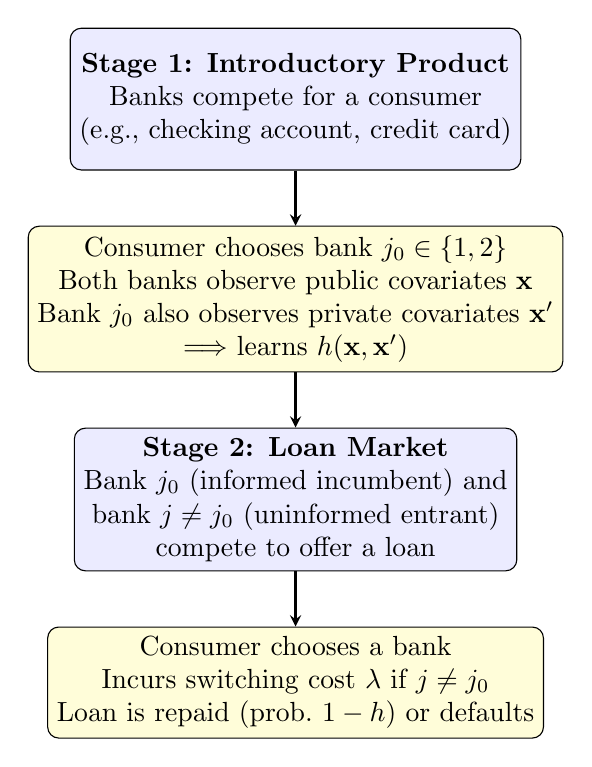
\begin{tikzpicture}[
    stage/.style={rectangle, draw, rounded corners, minimum width=5.5cm, minimum height=1.8cm, align=center, fill=blue!8},
    outcome/.style={rectangle, draw, rounded corners, minimum width=5.5cm, minimum height=1.2cm, align=center, fill=yellow!15},
    arrow/.style={->, thick, >=stealth}
]
\node[stage] (s1) {\textbf{Stage 1: Introductory Product}\\ Banks compete for a consumer\\(e.g., checking account, credit card)};
\node[outcome, below=0.7cm of s1] (o1) {Consumer chooses bank $j_0 \in \{1,2\}$\\Both banks observe public covariates $\mathbf{x}$\\Bank $j_0$ also observes private covariates $\mathbf{x}'$\\$\Longrightarrow$ learns $h(\mathbf{x},\mathbf{x}')$};
\node[stage, below=0.7cm of o1] (s2) {\textbf{Stage 2: Loan Market}\\ Bank $j_0$ (informed incumbent) and\\bank $j \neq j_0$ (uninformed entrant)\\compete to offer a loan};
\node[outcome, below=0.7cm of s2] (o2) {Consumer chooses a bank\\Incurs switching cost $\lambda$ if $j \neq j_0$\\Loan is repaid (prob.\ $1-h$) or defaults};

\draw[arrow] (s1) -- (o1);
\draw[arrow] (o1) -- (s2);
\draw[arrow] (s2) -- (o2);
\end{tikzpicture}
\end{center}

\medskip\noindent
\textbf{Stage~1.} Both banks compete to attract a consumer through an \emph{introductory product}---a checking account, a credit card, or a small initial loan. At this stage, neither bank has private information about the consumer's creditworthiness. Both banks observe publicly available borrower characteristics $\mathbf{x}$ (e.g., credit score, income, employment status). The consumer chooses one of the two banks (say bank~1). Through the ensuing relationship, bank~1 observes additional private characteristics $\mathbf{x}'$ (e.g., detailed repayment patterns, account activity, spending behavior) not available to bank~2, thereby learning the consumer's default probability~$h(\mathbf{x}, \mathbf{x}')$.

\medskip\noindent
\textbf{Two consequences of stage~1:}
\begin{enumerate}
    \item \textbf{Information asymmetry.} Bank~1 observes $(\mathbf{x}, \mathbf{x}')$ and therefore knows $h = h(\mathbf{x}, \mathbf{x}')$. Bank~2 observes only the public covariates $\mathbf{x}$ and therefore knows only the conditional distribution $F(h \mid \mathbf{x})$ of default probabilities, where the residual uncertainty arises from the unobserved private covariates $\mathbf{x}'$.
    \item \textbf{Switching costs.} The consumer develops a relationship with bank~1 (e.g., direct deposit, automatic payments, familiar digital platform). Switching to bank~2 for subsequent products imposes a cost $\lambda \geq 0$ on the consumer.
\end{enumerate}

\medskip\noindent
\textbf{Stage~2.} With bank~1 informed and the consumer partially locked in, the two banks compete to offer a loan. This is the \emph{cross-selling} stage: the introductory product was both a financial service in its own right and a mechanism for acquiring the informational advantage that shapes competition in the loan market. The incumbent can price-discriminate across borrower types, while the entrant sets a rate that may depend on the publicly observable covariates $\mathbf{x}$ but cannot condition on the private information $\mathbf{x}'$.

\medskip\noindent
\textbf{Solution approach: backward induction.} We solve the game by backward induction. Sections~\ref{sec:model}--\ref{sec:bank2profits} derive the stage~2 equilibrium, taking as given that one bank has acquired the customer (and hence the information and switching cost advantages). Section~\ref{sec:id} then establishes identification and develops the likelihood for estimation.


%===========================================================================
%  SECTION 2: STAGE 2 MODEL
%===========================================================================

\newpage
\section{Stage 2: Model}\label{sec:model}

There are two banks competing to lend to a consumer who is currently a client of bank~1 (from stage~1). Bank~1 (the \emph{informed/incumbent} bank) observes both $\mathbf{x}$ and $\mathbf{x}'$, and therefore knows the borrower's default probability $h = h(\mathbf{x}, \mathbf{x}')$. Bank~2 (the \emph{uninformed/entrant} bank) observes only the public covariates $\mathbf{x}$.

\subsection{Demand}

Consumer utility from borrowing from bank $j$ is:
\begin{align*}
    u_{i1} &= -\alpha\, r_{i1} + \varepsilon_{i1} \\
    u_{i2} &= -\alpha\, r_{i2} - \lambda + \varepsilon_{i2}
\end{align*}
where $r_{ij}$ is the interest rate, $\alpha > 0$ governs price sensitivity, $\lambda \geq 0$ is the switching cost incurred when moving to bank~2, and $\varepsilon_{ij}$ capture idiosyncratic preferences. The borrower chooses the bank with higher utility.

We write $s(r_1, r_2)$ for the probability that a borrower chooses the incumbent (bank~1). All results in Sections~\ref{sec:eq}--\ref{sec:logit} hold for any demand function satisfying Assumption~\ref{ass:demand}; Section~\ref{sec:logit} specializes to the logit.

\subsection{Information Structure and Covariates}\label{sec:info}

Each borrower is characterized by two sets of attributes:
\begin{itemize}
    \item \textbf{Public covariates} $\mathbf{x} \in \mathcal{X}$: observable by both banks (e.g., credit bureau score, income, employment status, age, existing debt levels).
    \item \textbf{Private covariates} $\mathbf{x}' \in \mathcal{X}'$: observable only by the home bank through the stage-1 relationship (e.g., detailed repayment patterns, account balances and volatility, spending behavior, direct deposit regularity).
\end{itemize}
The borrower's default probability is determined by both:
\begin{align}\label{eq:h_function}
    h = h(\mathbf{x}, \mathbf{x}')
\end{align}
Bank~1, having observed $(\mathbf{x}, \mathbf{x}')$, knows $h$ exactly. Bank~2, observing only $\mathbf{x}$, faces the conditional distribution of $h$ given $\mathbf{x}$, where the residual uncertainty arises from the unobserved $\mathbf{x}'$.

\medskip\noindent
\textbf{Convention.} \emph{The stage-2 analysis (Sections~\ref{sec:model}--\ref{sec:bank2profits}) is conducted conditional on a given realization of\/ $\mathbf{x}$. All distributions, densities, supports, and expectations are implicitly conditional on\/ $\mathbf{x}$: we write $F(h)$ for $F(h \mid \mathbf{x})$, $f(h)$ for $f(h \mid \mathbf{x})$, and $[h_{\min}, h_{\max}]$ for the $\mathbf{x}$-dependent support. Bank~2's rate $r_2$ is understood as $r_2(\mathbf{x})$. We make the conditioning on $\mathbf{x}$ explicit only where essential, particularly in the identification analysis (Section~\ref{sec:id}).}

\subsection{Types}

Conditional on public covariates $\mathbf{x}$, the default probability $h$ is distributed according to CDF $F(h \mid \mathbf{x})$ with density $f(h \mid \mathbf{x})$ on $[h_{\min}(\mathbf{x}), h_{\max}(\mathbf{x})] \subset (0,1)$, with $f(\cdot \mid \mathbf{x})$ bounded away from zero. The randomness in $h$ given $\mathbf{x}$ arises entirely from the unobserved private covariates $\mathbf{x}'$.

\subsection{Strategies}

Bank~1 observes each borrower's type $h$ and sets a type-contingent interest rate:
$$\sigma: [h_{\min}, h_{\max}] \to \mathbb{R}_+, \qquad h \mapsto \sigma(h)$$
Bank~2 does not observe $h$ but observes the public covariates $\mathbf{x}$, and sets an interest rate $r_2(\mathbf{x}) \in \mathbb{R}_+$ that may vary with $\mathbf{x}$ but is the same for all borrowers sharing the same public characteristics. Following our convention, we write $r_2$ for $r_2(\mathbf{x})$ throughout the stage-2 analysis.

\subsection{Profit Functions}

A loan to a type-$h$ borrower at rate $r$ yields expected revenue $(1-h)r$ against a unit cost of funds. The per-loan margin is $(1-h)r - 1$ and the break-even rate is $c(h) \equiv \frac{1}{1-h}$.

\medskip\noindent
Bank~1's expected profit from a type-$h$ borrower:
\begin{align}\label{eq:pi1}
    \pi_1(r_1;\, h,\, r_2) = \big[(1-h)\,r_1 - 1\big] \cdot s(r_1, r_2)
\end{align}

\medskip\noindent
Bank~2's expected profit (aggregated over types conditional on $\mathbf{x}$):
\begin{align}\label{eq:pi2}
    \pi_2(r_2;\, \sigma) = \int_{h_{\min}}^{h_{\max}} \big[(1-h)\,r_2 - 1\big] \cdot \big[1 - s(\sigma(h), r_2)\big] \, dF(h)
\end{align}
where the integral is over the conditional distribution $F(\cdot \mid \mathbf{x})$.

\subsection{Assumptions}

\begin{ass}[Type distribution]\label{ass:F}
For each $\mathbf{x} \in \mathcal{X}$, $F(\cdot \mid \mathbf{x})$ has support $[h_{\min}(\mathbf{x}), h_{\max}(\mathbf{x})] \subset (0,1)$, is absolutely continuous, and its density $f(\cdot \mid \mathbf{x})$ is bounded away from zero on its support.
\end{ass}

\begin{ass}[Demand regularity]\label{ass:demand}
The market share function $s: \mathbb{R}_+^2 \to (0,1)$ is $C^2$ and satisfies:
\begin{enumerate}
    \item[(i)] $s_1(r_1, r_2) < 0$ \quad (raising $r_1$ reduces bank~1's share);
    \item[(ii)] $s_2(r_1, r_2) > 0$ \quad (raising $r_2$ increases bank~1's share);
    \item[(iii)] $\ln s(r_1, r_2)$ is strictly concave in $r_1$ for each $r_2$ \quad (log-concavity).
\end{enumerate}
\end{ass}

\begin{ass}[Entrant concavity]\label{ass:pi2conc}
For any measurable $\sigma: [h_{\min}, h_{\max}] \to \mathbb{R}_+$, the aggregate profit $\pi_2(r_2; \sigma)$ is strictly concave in $r_2$. \footnote{\textcolor{red}{here one would need to 1. provide conditions of the primitives such that the profits of the second firm are concave and ideally relax it so that requires quas-concavity.}}
\end{ass}

\begin{remark}
Assumption~\ref{ass:demand}(iii) is equivalent to $s \cdot s_{11} < s_1^2$, i.e., the curvature condition $\frac{d^2}{dr_1^2}\ln s < 0$. Combined with the positive margin at the optimum, it ensures bank~1's profit is strictly quasi-concave in $r_1$, yielding a unique best response for each type. Assumption~\ref{ass:pi2conc} guarantees a unique optimal rate for bank~2. All three assumptions are satisfied by the logit demand (Section~\ref{sec:logit}).
\end{remark}

We define two objects that will appear throughout. The \emph{inverse semi-elasticity} of bank~$j$'s demand is:
\begin{align}\label{eq:markup_def}
    m_1(r_1, r_2) \equiv \frac{s(r_1, r_2)}{-s_1(r_1, r_2)}, \qquad m_2(r_1, r_2) \equiv \frac{1 - s(r_1, r_2)}{s_2(r_1, r_2)}
\end{align}
These are the standard ``markup functions'' from the IO pricing literature: each bank's markup above marginal cost equals $m_j$, as we show next.


%===========================================================================
%  SECTION 3: EQUILIBRIUM
%===========================================================================

\section{Pure Strategy Equilibrium}\label{sec:eq}

\begin{definition}[Pure Strategy Equilibrium]
A pure strategy equilibrium is a pair $(\sigma^*, r_2^*)$ such that:
\begin{enumerate}
    \item For each $h \in [h_{\min}, h_{\max}]$, \; $\sigma^*(h) \in \displaystyle\arg\max_{r_1 \geq 0} \; \pi_1(r_1;\, h,\, r_2^*)$.
    \item $r_2^*  \in \displaystyle\arg\max_{r_2 \geq 0} \; \pi_2(r_2;\, \sigma^*)$.
\end{enumerate}
where all distributions are conditional on $\mathbf{x}$, and $r_2^*$ is understood as $r_2^*(\mathbf{x})$.
\end{definition}

\begin{prop}[Equilibrium Characterization]\label{prop:char}
Under Assumptions~\ref{ass:F}--\ref{ass:pi2conc}, any interior pure strategy equilibrium $(\sigma^*, r_2^*)$ is characterized by the following system.

\medskip\noindent
\textbf{(i) Informed bank's pricing rule.} For each $h \in [h_{\min}, h_{\max}]$:
\begin{align}\label{eq:sigma}
    \boxed{\;\sigma^*(h) = \underbrace{\frac{1}{1-h}\vphantom{\Big|}}_{\text{break-even}} + \underbrace{m_1\!\big(\sigma^*(h),\, r_2^*\big)\vphantom{\Big|}}_{\text{markup}}\;}
\end{align}

\medskip\noindent
\textbf{(ii) Uninformed bank's pricing rule.} The rate $r_2^*$ satisfies:
\begin{align}\label{eq:r2foc}
    \int_{h_{\min}}^{h_{\max}} \left[(1-h)\big(1 - s(\sigma^*(h), r_2^*)\big) \;-\; s_2(\sigma^*(h), r_2^*)\, \big((1-h)\,r_2^* - 1\big)\right] dF(h) = 0
\end{align}
Equivalently:
\begin{align}\label{eq:r2star}
    \boxed{\;r_2^* = \frac{1}{1 - \hat{h}} + E_w\!\big[m_2\big]\;}
\end{align}
where $\hat{h} \equiv \frac{\int h\, s_2\, dF}{\int s_2\, dF}$ is the $s_2$-weighted average default probability, $E_w[m_2] \equiv \frac{\int m_2\, s_2\,(1-h)\, dF}{\int s_2\,(1-h)\, dF}$ is the weighted-average markup with weights $w(h) \propto s_2(\sigma^*(h), r_2^*)\,(1-h)\,f(h)$, and all functions are evaluated at $(\sigma^*(h), r_2^*)$.
\end{prop}

\begin{proof}
\textbf{Bank~1's first-order condition.} For each $h$, differentiate \eqref{eq:pi1} with respect to $r_1$:
\begin{align*}
    \frac{\partial \pi_1}{\partial r_1} = (1-h) \cdot s(r_1, r_2) + \big[(1-h)\,r_1 - 1\big] \cdot s_1(r_1, r_2) = 0
\end{align*}
Dividing by $s > 0$ and rearranging:
\begin{align*}
    (1-h) + \big[(1-h)\,r_1 - 1\big] \cdot \frac{s_1}{s} = 0 \qquad\Longrightarrow\qquad (1-h)\,r_1 - 1 = \frac{(1-h)\, s}{-s_1} = (1-h)\, m_1
\end{align*}
which yields \eqref{eq:sigma}. The second-order condition holds: by Assumption~\ref{ass:demand}(iii), $\ln s$ is strictly concave in $r_1$, so $s$ is log-concave; the product of the non-negative linear margin $(1-h)r_1 - 1$ and the log-concave share $s$ is strictly quasi-concave on the relevant domain, ensuring a unique maximizer.\footnote{At $r_1 = c(h) = \frac{1}{1-h}$ the margin is zero; the optimum lies strictly above this.}

\medskip\noindent
\textbf{Bank~2's first-order condition.} Differentiate \eqref{eq:pi2} with respect to $r_2$:
\begin{align*}
    \frac{d\pi_2}{dr_2} = \int_{h_{\min}}^{h_{\max}} \bigg[\underbrace{(1-h)\big(1-s\big)}_{\text{margin effect}} \;+\; \underbrace{\big[(1-h)\,r_2 - 1\big]\cdot(-s_2)}_{\text{share effect}}\bigg] dF(h) = 0
\end{align*}
using $\frac{\partial(1-s)}{\partial r_2} = -s_2$ (raising $r_2$ reduces bank~2's share). This is \eqref{eq:r2foc}.

\medskip\noindent
For the decomposition \eqref{eq:r2star}, rewrite \eqref{eq:r2foc} as:
\begin{align*}
    \int (1-h)(1-s)\, dF = \int s_2 \big[(1-h)\,r_2^* - 1\big]\, dF
\end{align*}
The left side equals $\int m_2 \cdot s_2 \,(1-h)\, dF$ (substituting $1-s = m_2 \cdot s_2$). Expanding the right side:
\begin{align*}
    r_2^* \int s_2(1-h)\, dF - \int s_2\, dF = \int m_2\, s_2\,(1-h)\, dF
\end{align*}
Hence:
\begin{align*}
    r_2^* = \frac{\int s_2\, dF}{\int s_2(1-h)\, dF} + \frac{\int m_2\, s_2\,(1-h)\, dF}{\int s_2\,(1-h)\, dF} = \frac{1}{1 - \hat{h}} + E_w[m_2] \qedhere
\end{align*}
\end{proof}

\begin{remark}[Parallel structure of pricing rules]\label{rem:parallel}
Both banks price at break-even plus a markup, but the nature of the markup differs:
\begin{itemize}
    \item Bank~1 prices \emph{type by type}: for each $h$, it sets break-even $c(h) = \frac{1}{1-h}$ plus the type-specific inverse semi-elasticity $m_1(\sigma^*(h), r_2^*)$.
    \item Bank~2 cannot condition on $h$, but can condition on the public covariates $\mathbf{x}$. For each $\mathbf{x}$, it prices at the break-even rate for an ``effective default probability'' $\hat{h}(\mathbf{x})$, plus a \emph{weighted average} of the type-specific markups $m_2(\sigma^*(h), r_2^*)$. The weights $w(h) \propto s_2 \cdot (1-h) \cdot f(h \mid \mathbf{x})$ emphasize types for which (a)~bank~2's demand is most price-sensitive (high $s_2$) and (b)~repayment probability is high (low $h$). Variation in $r_2^*$ across borrowers with different $\mathbf{x}$ is therefore generated by variation in $F(\cdot \mid \mathbf{x})$.
\end{itemize}
Both \eqref{eq:sigma} and \eqref{eq:r2star} are implicit equations: the markup on the right-hand side depends on the equilibrium rates.
\end{remark}



%===========================================================================
%  SECTION 5: LOGIT SPECIFICATION
%===========================================================================

\section{Logit Specification}\label{sec:logit}

We now specialize the general results to the logit demand arising from i.i.d.\ Type~I extreme value $\varepsilon_{ij}$:
\begin{align}\label{eq:logit_share}
    s(r_1, r_2) = \frac{\exp(-\alpha\, r_1)}{\exp(-\alpha\, r_1) + \exp(-\alpha\, r_2 - \lambda)} = \frac{1}{1 + \exp\!\big(\alpha(r_1 - r_2) - \lambda\big)}
\end{align}
This satisfies Assumptions~\ref{ass:demand} and~\ref{ass:pi2conc}.\footnote{$s_1 = -\alpha\,s(1-s) < 0$; $s_2 = \alpha\,s(1-s) > 0$; $\ln s = -\ln(1+e^{\alpha(r_1-r_2)-\lambda})$ is concave in $r_1$; and aggregate profit log-concavity in $r_2$ follows from Pr\'ekopa's theorem applied to the integrand.}

\subsection{Logit Inverse Semi-Elasticities}

The markup functions \eqref{eq:markup_def} take simple forms:
\begin{align}\label{eq:logit_m}
    m_1 = \frac{s}{-s_1} = \frac{s}{\alpha\, s(1-s)} = \frac{1}{\alpha(1-s)}, \qquad
    m_2 = \frac{1-s}{s_2} = \frac{1-s}{\alpha\, s(1-s)} = \frac{1}{\alpha\, s}
\end{align}

\subsection{Equilibrium Rates}

Substituting into Proposition~\ref{prop:char}:

\medskip\noindent
\textbf{Bank~1 (logit):}
\begin{align}\label{eq:sigma_logit}
    \sigma^*(h) = \frac{1}{1-h} + \frac{1}{\alpha\big(1 - s(\sigma^*(h), r_2^*)\big)}
\end{align}
For given $r_2^*$, this is an implicit equation for $\sigma^*(h)$ for each $h$.

\medskip\noindent
\textbf{Bank~2 (logit):}
\begin{align}\label{eq:r2_logit}
    r_2^* = \frac{1}{1 - \tilde{h}} + \frac{1}{\alpha}\cdot\frac{\displaystyle\int (1-s)(1-h)\, dF}{\displaystyle\int s\,(1-s)(1-h)\, dF}
\end{align}
where $\tilde{h} = \frac{\int h\, s(1-s)\, dF}{\int s(1-s)\, dF}$ and all shares are evaluated at $(\sigma^*(h), r_2^*)$.\footnote{This uses $s_2 = \alpha\,s(1-s)$, so the $s_2$-weights in \eqref{eq:r2star} become $s(1-s)$-weights.} The weights $\propto s(1-s)$ peak at $s = \frac{1}{2}$, emphasizing the most contested borrower types.

\begin{remark}[Source of variation in $r_2^*$ across borrowers]\label{rem:r2_variation}
In the data, we observe variation in the entrant's offered rate across borrowers. This variation is generated entirely by the public covariates $\mathbf{x}$: borrowers with different $\mathbf{x}$ have different conditional distributions $F(\cdot \mid \mathbf{x})$, which lead to different values of $\tilde{h}(\mathbf{x})$, different weighted-average markups, and hence different equilibrium rates $r_2^*(\mathbf{x})$. The private covariates $\mathbf{x}'$---which bank~2 cannot observe---generate within-$\mathbf{x}$ variation in $h$ but not in $r_2^*$.
\end{remark}


%===========================================================================
%  SECTION 6: UNINFORMED BANK PROFITS
%===========================================================================

\section{Uninformed Bank Profits}\label{sec:bank2profits}

In classical models without product differentiation, the uninformed bank earns zero expected profits. With logit demand, this is no longer the case: product differentiation (taste shocks) guarantees bank~2 strictly positive profits, though adverse selection erodes them relative to the symmetric-information benchmark.

\subsection{Strictly Positive Profits}

\begin{prop}[Bank~2 earns strictly positive profits]\label{prop:b2positive}
In any interior equilibrium of the logit model, $\pi_2(r_2^*; \sigma^*) > 0$.
\end{prop}

\begin{proof}
It suffices to exhibit a feasible rate yielding strictly positive profit, since the optimum $r_2^*$ does at least as well.

Set $\hat{r} = \frac{1}{1 - h_{\min}} + \varepsilon$ for some $\varepsilon > 0$. Then for every $h \in [h_{\min}, h_{\max}]$:
\begin{itemize}
    \item The margin $(1-h)\hat{r} - 1 \geq (1-h_{\min})\hat{r} - 1 > 0$ is strictly positive for the safest type and remains non-negative at least on a neighborhood $[h_{\min}, h_{\min} + \delta]$.\footnote{Specifically, $(1-h)\hat{r} > 1$ iff $h < 1 - 1/\hat{r}$, and $1 - 1/\hat{r} > h_{\min}$ by construction.}
    \item The logit share $1 - s(\sigma^*(h), \hat{r}) > 0$ for all $h$, since the logit never assigns zero probability.
\end{itemize}
Therefore the integrand in $\pi_2(\hat{r}; \sigma^*)$ is strictly positive on $[h_{\min}, h_{\min} + \delta]$ and bounded below, so $\pi_2(\hat{r}) > 0$. Since $r_2^*$ is optimal, $\pi_2(r_2^*) \geq \pi_2(\hat{r}) > 0$.
\end{proof}

\begin{remark}[Why classical models give zero profits]
In models without preference heterogeneity, demand is discontinuous: a borrower deterministically chooses the cheapest offer (adjusted for switching costs). The informed bank can always undercut the uninformed bank for profitable types, forcing bank~2 into a mixed strategy that earns zero expected profit (the standard Bertrand logic). Logit demand breaks this mechanism: even when bank~1 undercuts bank~2, some borrowers still choose bank~2 due to taste shocks. This residual demand provides a positive profit floor.
\end{remark}

\subsection{Profit Decomposition}

Bank~2's equilibrium profit can be decomposed by separating profitable from unprofitable borrower types. Define the \emph{break-even type for bank~2}:
\begin{align}\label{eq:hdagger}
    h^\dagger \equiv 1 - \frac{1}{r_2^*}
\end{align}
This is the default probability at which bank~2's per-loan margin $(1-h)r_2^* - 1$ equals zero. Types with $h < h^\dagger$ are profitable for bank~2; types with $h > h^\dagger$ generate losses.

\medskip\noindent
Then:
\begin{align}\label{eq:pi2_decomp}
    \pi_2(r_2^*; \sigma^*) = \underbrace{\int_{h_{\min}}^{h^\dagger} \big[(1-h)\,r_2^* - 1\big]\big(1-s\big)\, dF(h)}_{\displaystyle\pi_2^+ > 0 \;\text{(gains from safe types)}} \;+\; \underbrace{\int_{h^\dagger}^{h_{\max}} \big[(1-h)\,r_2^* - 1\big]\big(1-s\big)\, dF(h)}_{\displaystyle\pi_2^- < 0 \;\text{(losses from risky types)}}
\end{align}

The adverse selection pattern is directly visible here: bank~2's share $1-s(\sigma^*(h), r_2^*)$ is \emph{increasing} in $h$ (since $\sigma^*$ is increasing and $s_1 < 0$), so it captures a disproportionately large share of the loss-making risky types ($h > h^\dagger$) and a disproportionately small share of the profitable safe types ($h < h^\dagger$). The losses $\pi_2^-$ are the direct cost of the winner's curse.

\begin{remark}[Adverse selection cost]\label{rem:as_cost}
Define the \emph{adverse selection cost} as the profit gap relative to a hypothetical uninformed bank that faces the unconditional type distribution (i.e., whose share does not covary with $h$):
\begin{align}\label{eq:AS_cost}
    \Delta^{AS} \equiv \underbrace{\bar{s}_2 \int \big[(1-h)\,r_2^* - 1\big]\, dF(h)}_{\text{profit without adverse selection}} \;-\; \underbrace{\pi_2(r_2^*;\sigma^*)}_{\text{actual profit}}
\end{align}
where $\bar{s}_2 = \int (1-s)\, dF$ is bank~2's average market share. The first term computes bank~2's profit if its share were constant at $\bar{s}_2$ across all types (no adverse selection). By Chebyshev's inequality---since $1-s$ is increasing in $h$ and the margin $(1-h)r_2^* - 1$ is decreasing in $h$---the covariance between share and margin is negative, so $\Delta^{AS} > 0$: adverse selection strictly reduces bank~2's profit.
\end{remark}

\subsection{Comparative Statics}

\begin{prop}[Effect of $\alpha$ and $\lambda$ on bank~2 profits]\label{prop:b2compstat}
In the logit equilibrium:
\begin{enumerate}
    \item As $\alpha \to \infty$ (homogeneous preferences), $\pi_2 \to 0$. The model converges to the classical zero-profit result.
    \item As $\alpha \to 0$ (extreme differentiation), bank~2's market share approaches $\frac{1}{2}$ for all types and adverse selection vanishes. Bank~2's profit approaches that of a symmetric duopolist facing the average type.
    \item Higher switching costs $\lambda$ reduce bank~2's profit: they lower $1-s$ for all types, shrinking bank~2's share while amplifying the adverse selection pattern.
\end{enumerate}
\end{prop}

\begin{proof}[Proof sketch]
\emph{(1)} As $\alpha \to \infty$, the logit share converges to a step function: $s \to \mathbf{1}(\sigma^*(h) < r_2^* + \lambda/\alpha)$. For types where bank~1 undercuts, $1-s \to 0$ and bank~2 gets no demand. For types where bank~1 does not undercut, the informed bank has already set a rate above bank~2's (signaling that these are the risky types), so the margin $(1-h)r_2^* - 1$ tends to be negative or small. In the limit, bank~2 only attracts unprofitable borrowers, and $\pi_2 \to 0$.

\emph{(2)} As $\alpha \to 0$, rates become irrelevant for demand ($s \to e^{\lambda}/(1+e^{\lambda})$ for all types). Both banks earn the same margin from each type, there is no cream-skimming, and bank~2's profit converges to $\frac{1}{1+e^{\lambda}} \int [(1-h)r_2^* - 1]\, dF(h)$.

\emph{(3)} Increasing $\lambda$ shifts $s$ upward for all $(r_1, r_2)$ pairs, directly reducing $1-s(\sigma^*(h), r_2^*)$ for every type. This lowers both $\pi_2^+$ and $|\pi_2^-|$ in \eqref{eq:pi2_decomp}, but the effect on $\pi_2^+$ dominates because bank~2 already has low share among safe types where its margin is positive.
\end{proof}

\begin{remark}[What sustains bank~2's profits]
Bank~2's strictly positive profit rests entirely on product differentiation: the taste shocks $\varepsilon_{ij}$ ensure that some borrowers choose bank~2 even when it offers a higher rate than bank~1. These ``captive'' borrowers of bank~2 provide a profit floor that is absent in homogeneous-demand models. The economic content is that even an informationally disadvantaged competitor can survive and profit if borrowers have idiosyncratic preferences---whether due to branch location, service quality, digital platform, or relationship factors not captured by the interest rate.

However, bank~2's profit is bounded above: adverse selection ensures it earns less than it would under symmetric information, and switching costs compound this disadvantage. The uninformed bank is profitable but disadvantaged, with the degree of disadvantage governed by the interaction of $\alpha$ (substitutability) and $\lambda$ (lock-in).
\end{remark}


%===========================================================================
%  SECTION 7: IDENTIFICATION AND ESTIMATION
%===========================================================================

\newpage
\section{Identification and Estimation (Logit)}
\label{sec:id}

We now establish identification of the structural parameters, specializing to the logit demand from Section~\ref{sec:logit}. The analysis assumes the econometrician observes the public covariates $\mathbf{x}$ introduced in Section~\ref{sec:info}. In this section, we make the conditioning on $\mathbf{x}$ explicit and write $\sigma^*(h;\mathbf{x})$ for the $\mathbf{x}$-dependent pricing strategy and $r_2^*(\mathbf{x})$ for the entrant's rate.

\subsection{Estimation Primitives}\label{sec:primitives}

The structural parameters to be estimated are:

\begin{center}
\renewcommand{\arraystretch}{1.3}
\begin{tabular}{lll}
\toprule
\textbf{Parameter} & \textbf{Description} & \textbf{Dimension} \\
\midrule
$\alpha$ & Price sensitivity & Scalar \\
$\lambda$ & Switching cost & Scalar \\
$F(\cdot \mid \mathbf{x})$ & CDF of default probabilities, conditional on $\mathbf{x}$ & Function (for each $\mathbf{x}$) \\
\bottomrule
\end{tabular}
\end{center}

\medskip\noindent
In a parametric approach, $F(\cdot \mid \mathbf{x})$ is specified through a finite-dimensional parameterization---e.g., a Kumaraswamy$(a(\mathbf{x}), b(\mathbf{x}))$ distribution on $[h_{\min}(\mathbf{x}), h_{\max}(\mathbf{x})]$---so that the full parameter vector is finite. We first establish nonparametric identification---where $F(\cdot \mid \mathbf{x})$ is an infinite-dimensional object---and then discuss parametric estimation.

\medskip\noindent
All other model objects are \emph{derived} from these primitives:
\begin{itemize}
    \item The equilibrium strategies $\sigma^*(h; \mathbf{x})$ and $r_2^*(\mathbf{x})$ are determined by $(\alpha, \lambda, F(\cdot \mid \mathbf{x}))$ through the system \eqref{eq:sigma_logit}--\eqref{eq:r2_logit}.
    \item Market shares, markups, default rates, and profits follow.
\end{itemize}


\subsection{Observable Data}\label{sec:data}

For each borrower $i = 1, \ldots, N$, we observe:
\begin{center}
\renewcommand{\arraystretch}{1.3}
\begin{tabular}{lll}
\toprule
\textbf{Variable} & \textbf{Description} & \textbf{Values} \\
\midrule
$r_i^{\text{win}}$ & Interest rate charged by the chosen bank & $\mathbb{R}_+$ \\
$W_i$ & Identity of the chosen bank & $\{1, 2\}$ \\
$D_i$ & Default indicator & $\{0, 1\}$ \\
$\mathbf{x}_i$ & Public covariates & $\mathcal{X}$ \\
\bottomrule
\end{tabular}
\end{center}

\medskip\noindent
\textbf{What is NOT observed:}
\begin{enumerate}
    \item The borrower's true default probability $h_i$ (latent type)
    \item The private covariates $\mathbf{x}'_i$ (observed only by the home bank)
    \item The losing bank's rate offer
    \item Bank profits
\end{enumerate}

\begin{remark}[Data structure with covariates]\label{rem:data_x}
When bank~2 wins ($W_i = 2$), the winning rate $r_i^{\text{win}} = r_2^*(\mathbf{x}_i)$ varies across borrowers with different public covariates. Conditional on $\mathbf{x}$, however, $r_2^*(\mathbf{x})$ is the same for all bank~2 winners---this is the identifying feature from the model without covariates, now applied within each $\mathbf{x}$-stratum. When bank~1 wins ($W_i = 1$), the winning rate $r_i^{\text{win}} = \sigma^*(h_i; \mathbf{x}_i)$ varies due to both $h_i$ and $\mathbf{x}_i$.
\end{remark}


\subsection{Identification Argument}\label{sec:id_arg}

We establish identification sequentially: each step uses objects identified in previous steps.

\begin{thm}[Identification with observable covariates]\label{thm:id}
The structural parameters $(\alpha, \lambda, F(\cdot|\mathbf{x}))$ are identified from the joint distribution of $(r_i^{\textup{win}}, W_i, D_i, \mathbf{x}_i)$.
\end{thm}

The proof proceeds in four steps, each conditional on $\mathbf{x}$.


\subsubsection{Step 1: Identification of $r_2^*(\mathbf{x})$}

\begin{prop}\label{prop:id_r2}
The entrant's rate function $r_2^*(\mathbf{x})$ is identified from the data.
\end{prop}

\begin{proof}
For each $\mathbf{x}$, bank~2 plays a single rate $r_2^*(\mathbf{x})$ for all borrowers with public covariates $\mathbf{x}$. When $W_i = 2$ and $\mathbf{x}_i = \mathbf{x}$, the winning rate is $r_i^{\text{win}} = r_2^*(\mathbf{x})$. Therefore $r_2^*(\mathbf{x})$ is the common value of $r_i^{\text{win}}$ among all bank~2 winners with covariates $\mathbf{x}$.
\end{proof}

\begin{remark}
When $\mathbf{x}$ is continuous, $r_2^*(\mathbf{x})$ can be estimated as a nonparametric regression of $r_i^{\text{win}}$ on $\mathbf{x}_i$ among bank~2 winners. The model predicts that this regression has conditional variance zero (all bank~2 winners with the same $\mathbf{x}$ receive the same rate); departures from this prediction indicate model misspecification.
\end{remark}


\subsubsection{Step 2: Identification of $\sigma^*(\cdot\,;\mathbf{x})$ and the mapping $h \leftrightarrow r_1$}

\begin{prop}\label{prop:id_sigma}
For each $\mathbf{x}$, the informed bank's pricing function $\sigma^*(\cdot\,;\mathbf{x})$ and its inverse $\tau(\cdot\,;\mathbf{x}) = \sigma^{*-1}(\cdot\,;\mathbf{x})$ are identified from $(r_i^{\textup{win}}, D_i)$ conditional on $W_i = 1$ and $\mathbf{x}_i = \mathbf{x}$.
\end{prop}

\begin{proof}
When bank~1 wins, the observed rate is $r_i^{\text{win}} = \sigma^*(h_i; \mathbf{x}_i)$ and the default outcome is $D_i \sim \text{Bernoulli}(h_i)$. Since default is conditionally independent of rates and covariates given $h_i$:
\begin{align}\label{eq:id_h_from_D}
    E[D_i \mid r_i^{\text{win}} = r,\; W_i = 1,\; \mathbf{x}_i = \mathbf{x}] = h_i = \tau(r; \mathbf{x})
\end{align}
This identifies the inverse pricing function: the conditional default rate at each observed rate $r$ among bank~1 winners with covariates $\mathbf{x}$ equals the default probability of the type that receives rate $r$ under the equilibrium $\sigma^*(\cdot\,; \mathbf{x})$.\footnote{In finite samples, $E[D|r, W\!=\!1, \mathbf{x}]$ is estimated nonparametrically, e.g., by kernel regression of $D_i$ on $r_i^{\text{win}}$ among bank~1 winners with covariates close to $\mathbf{x}$.}
\end{proof}

\begin{remark}[Why conditioning on $\mathbf{x}$ is essential in Step~2]\label{rem:x_essential}
Two borrowers with the same bank~1 rate $r$ but different $\mathbf{x}$ will generally have different types, because the inverse function $\tau(r; \mathbf{x})$ depends on $\mathbf{x}$ through $r_2^*(\mathbf{x})$. Intuitively, a rate of $r_1 = 8\%$ offered to a borrower with a high credit score ($\mathbf{x}$ implying low $r_2^*$, hence high competitive pressure) reveals a different type than the same rate offered to a borrower with a low credit score ($\mathbf{x}$ implying high $r_2^*$, hence low competitive pressure). Omitting $\mathbf{x}$ from the conditioning would conflate these types.
\end{remark}

\medskip\noindent
After Step~2, for each bank~1 winner with covariates $\mathbf{x}$ we can compute:
\begin{itemize}
    \item $h_i = \tau(r_i^{\text{win}}; \mathbf{x}_i)$: the inferred type
    \item $m_i \equiv r_i^{\text{win}} - \frac{1}{1-h_i} = \sigma^*(h_i;\mathbf{x}_i) - c(h_i)$: the observed \emph{markup}
    \item $\Delta_i \equiv r_i^{\text{win}} - r_2^*(\mathbf{x}_i) = \sigma^*(h_i;\mathbf{x}_i) - r_2^*(\mathbf{x}_i)$: the \emph{rate gap}
\end{itemize}
These are data objects, computed without knowledge of $\alpha$ or $\lambda$.


\subsubsection{Step 3: Joint identification of $\alpha$ and $\lambda$}

This is the key step. The equilibrium FOC imposes a restriction linking the data objects $m(h;\mathbf{x})$ and $\Delta(h;\mathbf{x})$ to the structural parameters $\alpha$ and $\lambda$.

\begin{prop}\label{prop:id_alpha_lambda}
The parameters $\alpha$ and $\lambda$ are jointly identified from the pricing function $\sigma^*(\cdot\,;\mathbf{x})$, the break-even rate $c(h) = \frac{1}{1-h}$, and the entrant rate $r_2^*(\mathbf{x})$.
\end{prop}

\begin{proof}
\textbf{Deriving the identifying restriction.} From the logit FOC \eqref{eq:sigma_logit}, the markup satisfies:
\begin{align*}
    m(h; \mathbf{x}) = \sigma^*(h; \mathbf{x}) - \frac{1}{1-h} = \frac{1}{\alpha(1-s)}
\end{align*}
Substituting the logit share $1-s = \frac{e^{\alpha\Delta(h;\mathbf{x})-\lambda}}{1+e^{\alpha\Delta(h;\mathbf{x})-\lambda}}$:
\begin{align*}
    m(h; \mathbf{x}) = \frac{1}{\alpha}\left(e^{\lambda - \alpha\Delta(h;\mathbf{x})} + 1\right)
\end{align*}
Rearranging and taking logarithms:
\begin{align}\label{eq:id_linear}
    \boxed{\;\ln\!\big(\alpha\, m(h;\mathbf{x}) - 1\big) = \lambda - \alpha\, \Delta(h;\mathbf{x})\;}
\end{align}
This must hold for \emph{every} $(h, \mathbf{x})$ pair. Both $m(h;\mathbf{x})$ and $\Delta(h;\mathbf{x})$ are known data objects (from Steps 1--2), while $\alpha$ and $\lambda$ are the two unknowns.

\medskip\noindent
\textbf{Separation of $\alpha$ and $\lambda$.} Evaluating \eqref{eq:id_linear} at any two distinct pairs $(h_a, \mathbf{x}_a)$ and $(h_b, \mathbf{x}_b)$ and subtracting:
\begin{align}\label{eq:id_alpha}
    \ln\frac{\alpha\, m(h_a;\mathbf{x}_a) - 1}{\alpha\, m(h_b;\mathbf{x}_b) - 1} = \alpha\,\big(\Delta(h_b;\mathbf{x}_b) - \Delta(h_a;\mathbf{x}_a)\big)
\end{align}
This is a single equation in the single unknown $\alpha$, since all other quantities are data. The two pairs can come from:
\begin{enumerate}
    \item[(a)] Different types $h_a \neq h_b$ within the same $\mathbf{x}$ (as in the model without covariates), or
    \item[(b)] The same type $h$ across different $\mathbf{x}$ values (new source of variation), or
    \item[(c)] Any combination of $(h, \mathbf{x})$ variation.
\end{enumerate}

\medskip\noindent
\textbf{Uniqueness.} The uniqueness argument is identical to the model without covariates. Define $\psi(\alpha) \equiv \ln(\alpha m_a - 1) - \ln(\alpha m_b - 1) - \alpha(\Delta_b - \Delta_a)$ where $m_j = m(h_j; \mathbf{x}_j)$ and $\Delta_j = \Delta(h_j; \mathbf{x}_j)$, with $m_a > m_b$ and $\Delta_a < \Delta_b$. Then $\psi$ is continuous with $\psi(\alpha) \to +\infty$ as $\alpha \downarrow 1/m_b$, $\psi(\alpha) \to -\infty$ as $\alpha \to \infty$, and $\psi' < 0$, yielding a unique root.

\medskip\noindent
\textbf{Recovery of $\lambda$.} Given $\alpha$, substitute into \eqref{eq:id_linear} at any $(h, \mathbf{x})$:
\begin{align}\label{eq:id_lambda}
    \lambda = \ln\!\big(\alpha\, m(h;\mathbf{x}) - 1\big) + \alpha\, \Delta(h;\mathbf{x})
\end{align}
The fact that this must be constant across \emph{all} $(h, \mathbf{x})$ pairs is overidentifying.
\end{proof}

\begin{remark}[Intuition for separate identification]\label{rem:id_intuition}
The identifying restriction \eqref{eq:id_linear} states that $\ln(\alpha m - 1)$ is an affine function of $\Delta$ with slope $-\alpha$ and intercept $\lambda$:
\begin{itemize}
    \item \textbf{$\alpha$ governs the slope:} higher price sensitivity means the markup responds more steeply to the rate gap.
    \item \textbf{$\lambda$ governs the intercept:} switching costs shift bank~1's markup uniformly upward.
\end{itemize}
Cross-$\mathbf{x}$ variation in $r_2^*(\mathbf{x})$ shifts the rate gap $\Delta$ without changing the slope--intercept relationship, providing additional leverage for identification.
\end{remark}


\subsubsection{Step 4: Identification of $F(h \mid \mathbf{x})$}

\begin{prop}\label{prop:id_F}
For each $\mathbf{x}$, the conditional type distribution $F(h \mid \mathbf{x})$ is nonparametrically identified.
\end{prop}

\begin{proof}
With $\alpha, \lambda$ known (from Step~3), the market share for each type conditional on $\mathbf{x}$ is:
\begin{align}\label{eq:id_s_known}
    s(h; \mathbf{x}) \equiv s(\sigma^*(h;\mathbf{x}), r_2^*(\mathbf{x})) = \frac{1}{1 + \exp\!\big(\alpha\,\Delta(h;\mathbf{x}) - \lambda\big)}
\end{align}
which is a known function of $h$ (since $\sigma^*$ and $r_2^*$ are identified).

Among bank~1 winners with covariates $\mathbf{x}$, the density of types is the selection-weighted density:
\begin{align}\label{eq:id_f1}
    f_{h|W=1,\mathbf{x}}(h) = \frac{s(h; \mathbf{x})\, f(h \mid \mathbf{x})}{\Pr(W_i = 1 \mid \mathbf{x}_i = \mathbf{x})}
\end{align}
The left side is estimable from the data: among bank~1 winners with covariates $\mathbf{x}$, the inferred types $h_i = \tau(r_i^{\text{win}}; \mathbf{x})$ (Step~2) have empirical density that estimates $f_{h|W=1,\mathbf{x}}$. Inverting:
\begin{align}\label{eq:id_f_recovered}
    f(h \mid \mathbf{x}) = \frac{f_{h|W=1,\mathbf{x}}(h) \cdot \Pr(W_i = 1 \mid \mathbf{x}_i = \mathbf{x})}{s(h; \mathbf{x})}
\end{align}
Since $s(h; \mathbf{x}) > 0$ for all $h$ (logit shares are strictly interior), this is well-defined. The aggregate probability $\Pr(W_i = 1 \mid \mathbf{x})$ is the sample share of bank~1 winners among borrowers with covariates $\mathbf{x}$.
\end{proof}


\subsection{Overidentification from Cross-$\mathbf{x}$ Variation}\label{sec:overid_x}

The model with observable covariates generates substantially richer overidentifying restrictions than the model without covariates.

\subsubsection{Joint linearity across all $(h, \mathbf{x})$ pairs}

The identifying restriction \eqref{eq:id_linear} must hold for \emph{all} $(h, \mathbf{x})$ pairs. In the $(\Delta, \ln(\alpha m - 1))$-plane:
\begin{itemize}
    \item \textbf{Within-$\mathbf{x}$ variation:} for a fixed $\mathbf{x}$, different types $h$ trace out points along the line. This is the same overidentification as in the model without covariates.
    \item \textbf{Cross-$\mathbf{x}$ variation:} different values of $\mathbf{x}$ generate different $r_2^*(\mathbf{x})$, shifting the $\Delta$-schedule. The key prediction: these shifted points must still lie on the \emph{same} line (same slope $-\alpha$ and same intercept $\lambda$). This cross-$\mathbf{x}$ linearity is a new and powerful testable restriction.
\end{itemize}
Departures from joint linearity indicate model misspecification: for example, heterogeneity in $\alpha$ or $\lambda$ across borrower types, or failure of the logit functional form.

\subsubsection{Adverse selection within each $\mathbf{x}$-stratum}

For each $\mathbf{x}$, the model predicts:
\begin{align*}
    E[D_i \mid W_i = 1, \mathbf{x}_i = \mathbf{x}] < E[D_i \mid \mathbf{x}_i = \mathbf{x}] < E[D_i \mid W_i = 2, \mathbf{x}_i = \mathbf{x}]
\end{align*}
Bank~2 winners should have a strictly higher default rate than bank~1 winners \emph{within every $\mathbf{x}$-stratum}. The magnitude of the gap is pinned down by the estimated $(\alpha, \lambda, F(\cdot|\mathbf{x}))$.

\subsubsection{Bank~2 FOC consistency}

Having identified $\alpha, \lambda, F(\cdot|\mathbf{x})$, the model predicts $r_2^*(\mathbf{x})$ for each $\mathbf{x}$ via the FOC \eqref{eq:r2_logit}. This predicted rate can be compared to the directly-observed $r_2^*(\mathbf{x})$ (from Step~1) for each $\mathbf{x}$ value, providing a family of model-fit checks indexed by $\mathbf{x}$.


\subsection{Likelihood-Based Estimation}\label{sec:estimation}

For parametric estimation, condition on $\mathbf{x}_i$ and specify $F(\cdot \mid \mathbf{x};\theta_F)$ through a parametric family indexed by a finite-dimensional parameter $\theta_F$. The full parameter vector is $\theta = (\alpha, \lambda, \theta_F)$.

\subsubsection{Likelihood function}

\paragraph{Bank~1 wins ($W_i = 1$):} The winning rate $r_i^{\text{win}} = \sigma^*(h_i; \mathbf{x}_i)$ reveals $h_i = \tau(r_i^{\text{win}}; \mathbf{x}_i)$:
\begin{align}\label{eq:L1}
    \mathcal{L}_i^{(1)} = \underbrace{f\!\big(\tau(r_i^{\text{win}}; \mathbf{x}_i) \mid \mathbf{x}_i;\theta_F\big) \cdot |\tau'(r_i^{\text{win}}; \mathbf{x}_i)|}_{\text{density of rate}} \cdot \underbrace{s\!\big(r_i^{\text{win}}, r_2^*(\mathbf{x}_i)\big)}_{\text{prob.\ bank~1 chosen}} \cdot \underbrace{h_i^{D_i}(1-h_i)^{1-D_i}}_{\text{default probability}}
\end{align}
where $h_i = \tau(r_i^{\text{win}}; \mathbf{x}_i)$ and $|\tau'|$ is the Jacobian from the change of variables $h \to r_1$.

\paragraph{Bank~2 wins ($W_i = 2$):} The winning rate is $r_i^{\text{win}} = r_2^*(\mathbf{x}_i)$ and $h_i$ is unobserved:
\begin{align}\label{eq:L2}
    \mathcal{L}_i^{(2)} = \int_{h_{\min}(\mathbf{x}_i)}^{h_{\max}(\mathbf{x}_i)} \underbrace{\big(1-s(\sigma^*(h;\mathbf{x}_i), r_2^*(\mathbf{x}_i))\big)}_{\text{prob.\ bank~2 chosen}} \cdot \underbrace{h^{D_i}(1-h)^{1-D_i}}_{\text{default prob.}} \cdot f(h \mid \mathbf{x}_i;\theta_F)\, dh
\end{align}

\paragraph{Full log-likelihood:}
\begin{align}\label{eq:loglik}
    \ell(\theta) = \sum_{i=1}^N \Big[\mathbf{1}(W_i=1)\ln \mathcal{L}_i^{(1)} + \mathbf{1}(W_i=2)\ln \mathcal{L}_i^{(2)}\Big]
\end{align}

\subsubsection{Estimation procedure}

\begin{enumerate}
    \item \textbf{Fix $\theta = (\alpha, \lambda, \theta_F)$.} For each unique $\mathbf{x}$ value in the data (or on a grid), solve the equilibrium: compute $\sigma^*(h; \mathbf{x}; \theta)$ and $r_2^*(\mathbf{x};\theta)$ from the system \eqref{eq:sigma_logit}--\eqref{eq:r2_logit} numerically.
    \item \textbf{Evaluate the log-likelihood} $\ell(\theta)$ using \eqref{eq:L1}--\eqref{eq:L2}.
    \item \textbf{Maximize} $\ell(\theta)$ over $\theta$ using numerical optimization.
    \item \textbf{Standard errors} from the inverse Hessian or bootstrap.
\end{enumerate}

\begin{remark}[Computational structure]
For bank~1 winners, the likelihood is in closed form (no integral) because the winning rate reveals the type. For bank~2 winners, a one-dimensional numerical integral over $h$ is required. The equilibrium must be re-solved for each unique $\mathbf{x}$ at each candidate $\theta$. If $\mathbf{x}$ is discrete with $K$ levels, this requires $K$ equilibrium solves per likelihood evaluation; if continuous, it can be handled by solving on a grid of $\mathbf{x}$-values and interpolating.
\end{remark}


\subsection{Summary of Identification Logic}

\begin{center}
\renewcommand{\arraystretch}{1.4}
\begin{tabular}{lll}
\toprule
\textbf{Object} & \textbf{Identified from} & \textbf{Step} \\
\midrule
$r_2^*(\mathbf{x})$ & Winning rate when $W_i = 2$, conditional on $\mathbf{x}$ & 1 \\
$\sigma^*(h;\mathbf{x})$, $\tau(r;\mathbf{x})$ & $E[D|r, W\!=\!1, \mathbf{x}]$ (defaults reveal types) & 2 \\
$\alpha$ & Eq.\ \eqref{eq:id_alpha}: markup curvature across $(h,\mathbf{x})$ pairs & 3 \\
$\lambda$ & Eq.\ \eqref{eq:id_lambda}: markup level given $\alpha$ & 3 \\
$F(h|\mathbf{x})$ & Selection-corrected type distribution, for each $\mathbf{x}$ & 4 \\
\bottomrule
\end{tabular}
\end{center}


\end{document}
